\chapter{Projektverlauf und Meilensteine} \label{ch:projektverlauf}
Dieses Kapitel beschreibt die einzelnen Entwicklungsschritte und die dadurch erreichten Meilensteine unserer Sprints.

\section{Anforderungs- und Risikoanalyse}
Im ersten Sprint haben wir uns mit der Definition der Anforderungen (Requirements) beschäftigt. 
Ziel war es, festzulegen, welche Aspekte unser Projekt abdecken soll und welche Eigenschaften möglicherweise unrealistisch oder optional sind, um einen klaren Fokus zu setzen. 
Eine detailliertere Beschreibung der Anforderungen findet sich in Kapitel \ref{ch:projektziele}.\\
\\
Gleichzeitig mit der Festlegung der Anforderungen haben wir uns ebenfalls mit den daraus resultierenden Risiken auseinandergesetzt. 
Hierbei stand die Frage im Vordergrund, welche Fehlschläge am wahrscheinlichsten und gravierendsten sein könnten. 
Besonders besorgniserregend waren die Risiken in Bezug auf die Beschaffung der Logdateien und den Datenschutz. 
Eine genauere Beschreibung der Risikobewertung findet sich ebenfalls in Kapitel \ref{ch:Risikoanalyse}.

\section{Programmentwurf und Architekturentwurf}
Unser zweiter großer Meilenstein war die Ausarbeitung eines möglichen Programmentwurfs, also der strukturelle Aufbau des Programms.\\
\\
Der Entwurf des Programms sowie die Architektur von \gls{cybrail} basieren auf einer klaren Strukturierung der Funktionalitäten, um eine effiziente und erweiterbare Lösung zu gewährleisten. 
Im folgenden Abschnitt wird der Architekturentwurf näher erläutert, gefolgt von einem detaillierten Blick auf die wichtigsten Klassen und deren Interaktionen.

\subsection{Architekturentwurf}

Das Architekturdiagramm (siehe Abbildung \ref{fig:Architektur}) verdeutlicht die modulare Struktur des Log Processing Systems von CYBRAIL, das in zwei Hauptbereiche unterteilt ist: den \textit{InfoPrep}-Bereich und die \textit{TestingPipeline}.

Im \textbf{InfoPrep}-Bereich werden die eingehenden Logdaten vorverarbeitet. Der wesentliche verbleibende Bestandteil dieses Bereichs ist der \texttt{LogParser}, der die Logs in ein standardisiertes JSON-Format umwandelt, das für die weitere Verarbeitung verwendet wird. Die vorverarbeiteten Daten werden dann an die \textbf{TestingPipeline} weitergeleitet.

Die \textbf{TestingPipeline} führt die eigentlichen Tests auf den vorverarbeiteten Logs durch. Dabei kommen verschiedene Module zum Einsatz, die auf unterschiedliche Anomalien testen. Diese umfassen: \begin{itemize} \item \textbf{MLAnomalyDetector:} Nutzt Machine-Learning-Modelle, wie zum Beispiel zur Erkennung automatischen Tippens (FastTyping Detection). \item \textbf{RuleBasedAnomalyDetector:} Führt regelbasierte Anomalieerkennungen durch, wie die VM-Erkennung (VM Detection) oder die Erkennung mehrerer Bildschirme (Number of Displays Detection). \end{itemize}

Am Ende des Prozesses werden alle Ergebnisse von der \texttt{ResultAggregator}-Komponente gesammelt und zu einem Gesamtbericht zusammengeführt. Dieser Bericht wird anschließend durch die \texttt{Output}-Komponente ausgegeben oder gespeichert.

Durch diese modulare Architektur kann das System flexibel erweitert werden, indem neue Testmodule hinzugefügt oder bestehende angepasst werden. Ebenso bleibt das Parsing der Logs flexibel, um neue Logformate zu unterstützen.

\begin{landscape} 
  \begin{figure}[h] \centering 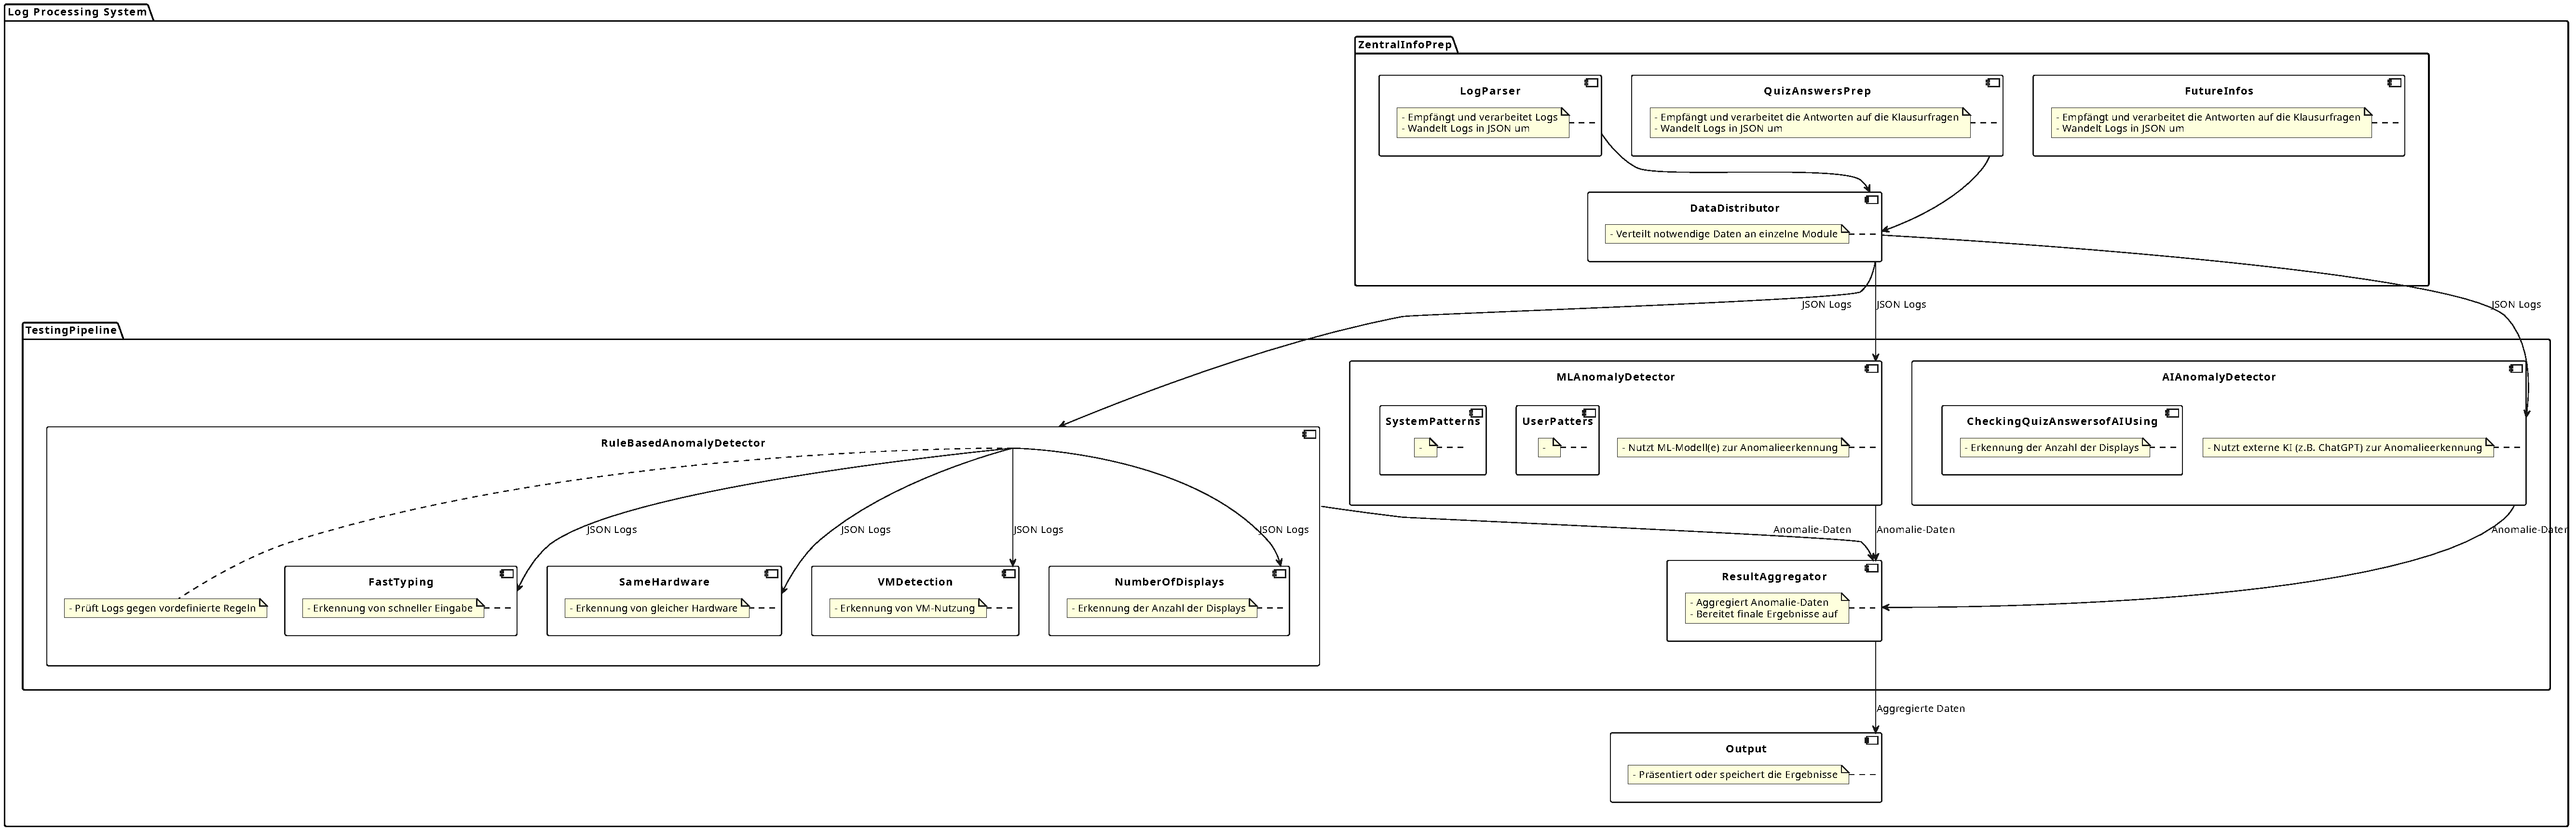
\includegraphics[width=1.5\textwidth]{figures/CybrailArchitektur.pdf} \caption{Architekturdiagramm des Log Processing Systems von CYBRAIL} \label{fig:Architektur} \end{figure} \end{landscape}

\subsection{Programmentwurf}

Das Klassendiagramm (siehe Abbildung \ref{fig:Klassen}) zeigt das Log Processing System von CYBRAIL aus einer objektorientierten Perspektive. Die zentralen Klassen und deren Funktionen sind: \begin{itemize} \item \texttt{LogParser:} Verantwortlich für das Einlesen und Umwandeln von Logdateien in das JSON-Format. \item \texttt{DataDistributor:} Verteilt die vorverarbeiteten Daten an die verschiedenen Testmodule in der TestingPipeline. \item \texttt{RuleBasedAnomalyDetector:} Prüft die Logs auf Basis vordefinierter Regeln, wie der Erkennung von VM-Nutzung oder mehreren Bildschirmen. \item \texttt{MLAnomalyDetector:} Setzt Machine-Learning-Modelle zur Erkennung von Anomalien, wie schnellem Tippen, ein. \item \texttt{ResultAggregator:} Aggregiert die Ergebnisse aller Anomaliedetektoren und erstellt einen finalen Bericht. \item \texttt{Output:} Gibt die gesammelten Ergebnisse aus oder speichert sie. \end{itemize}

Die modulare Struktur des Systems ermöglicht es, die einzelnen Testmodule unabhängig voneinander zu entwickeln und zu erweitern, ohne das Gesamtsystem zu beeinträchtigen. Dies erleichtert auch zukünftige Anpassungen und Erweiterungen.

\begin{landscape} \begin{figure}[h] \centering 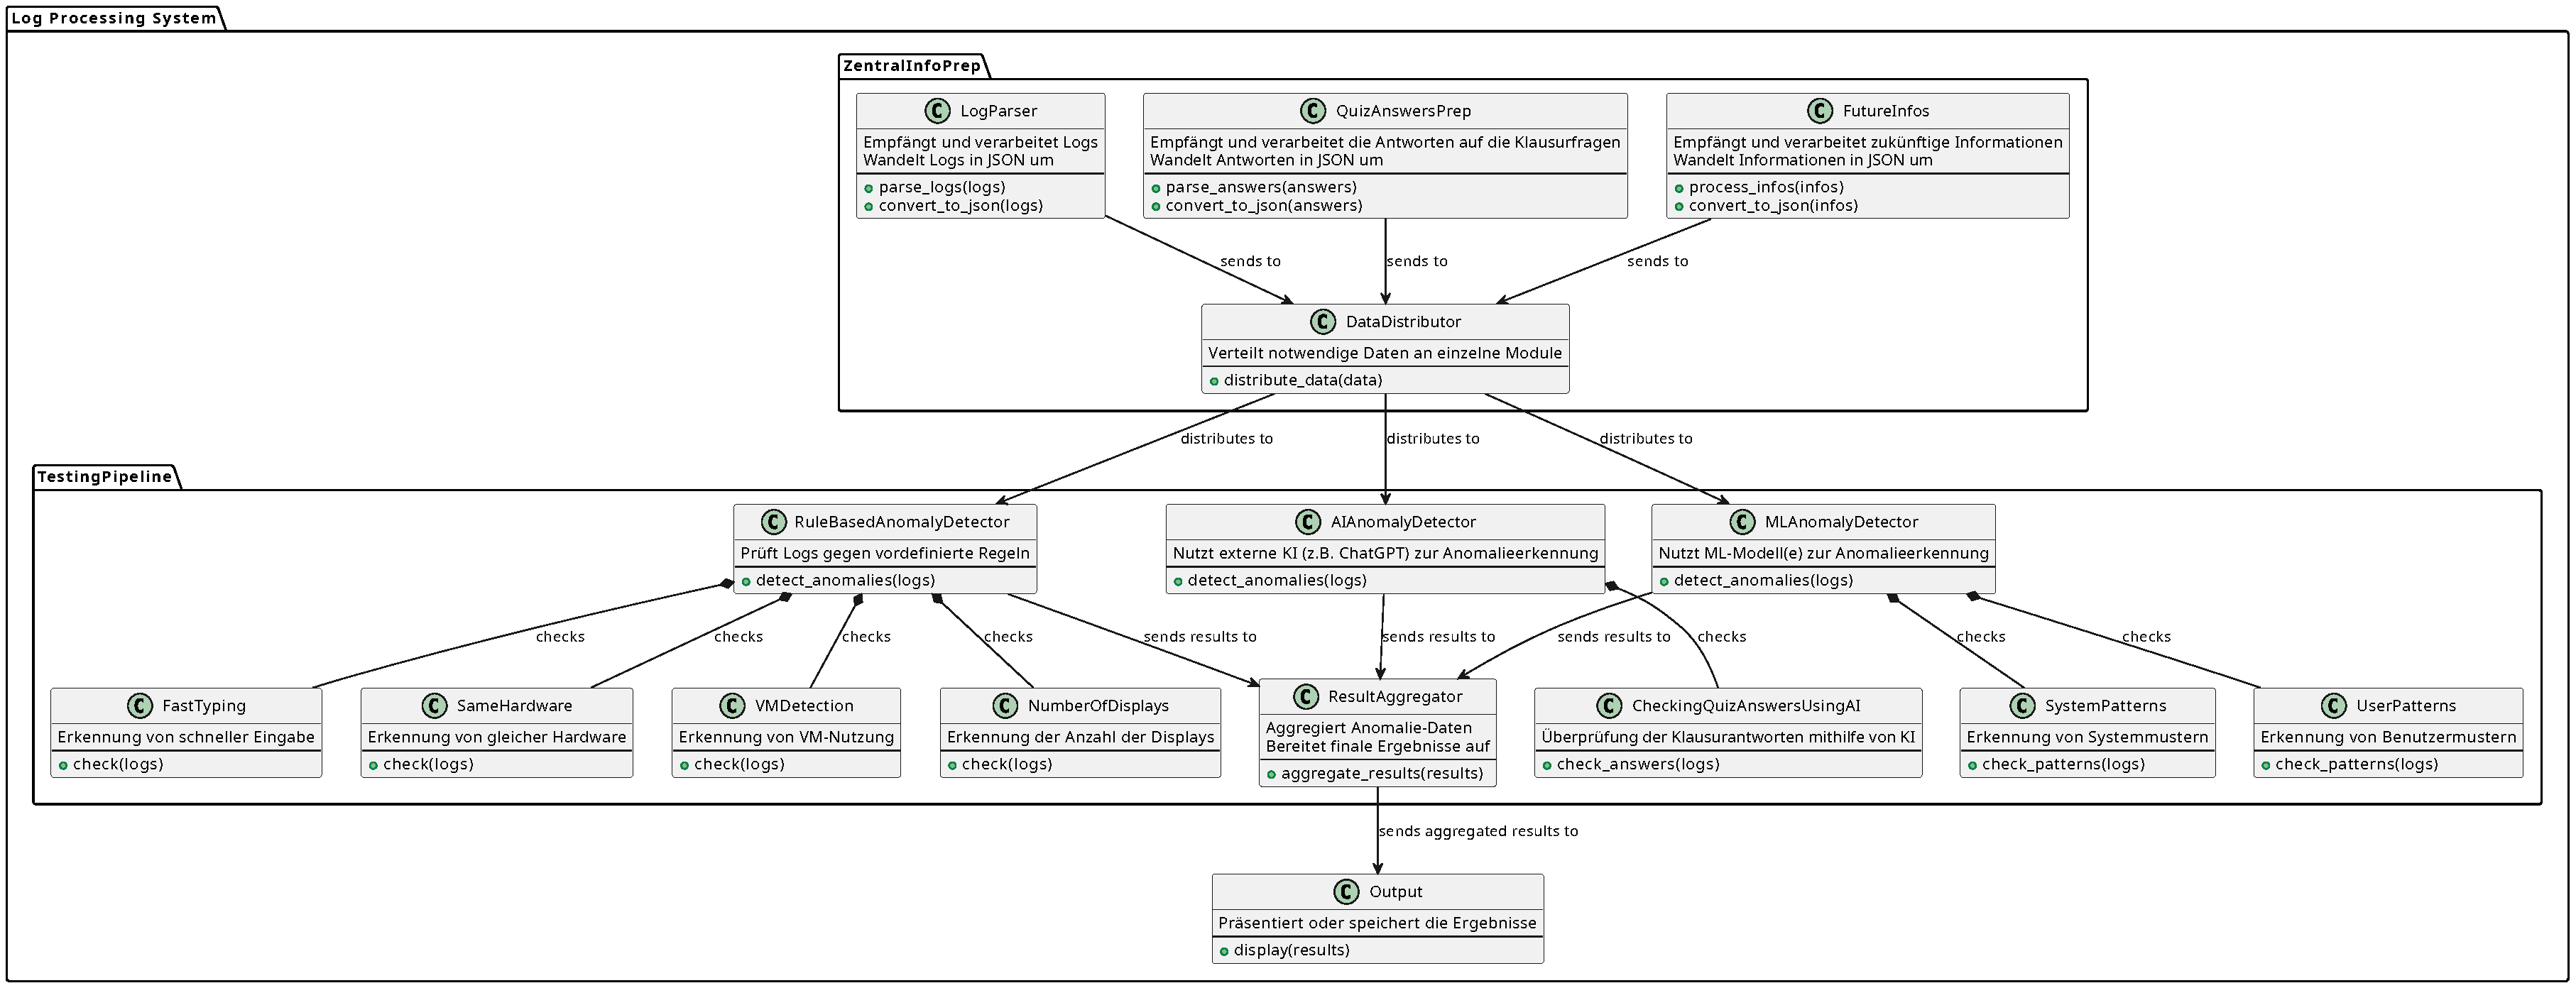
\includegraphics[width=1.5\textwidth]{figures/CybrailClassdiagramm.pdf} \caption{Klassendiagramm des Log Processing Systems von CYBRAIL} \label{fig:Klassen} \end{figure} \end{landscape}

\subsection{Zusammenfassung}

Der Architektur- und Programmentwurf von CYBRAIL zeigt einen modularen Ansatz, der es ermöglicht, das System flexibel zu erweitern und an neue Anforderungen anzupassen. Die klare Trennung von Vorverarbeitung, Anomalieerkennung und Ergebnisaggregation gewährleistet, dass das System sowohl effizient arbeitet als auch gut skalierbar ist. Neue Testmodule und Anpassungen am Logparsing können einfach integriert werden, ohne die bestehende Systemarchitektur zu beeinflussen.

\section{Logparsing und erstes MVP}
Zu Beginn war es wichtig, die eigentlichen Daten, mit denen wir arbeiten wollten, in ein computerlesbares Format zu bringen und somit ein erstes \gls{mvp} zu erstellen.\\
\\
Wir haben einen modularen Ansatz entwickelt, der mithilfe eines Strategy Patterns die unterschiedlichen Arten von Logs – sowohl die der \gls{seb} als auch andere Logtypen – unterscheiden kann und einfach um neue Logtypen erweiterbar ist. 
Dieses Modul nimmt alle Logdateien als Input, identifiziert den Logtyp anhand des Dateinamens und wendet schließlich die passende Strategie an, um das Log in parsierbare \gls{json}-Dateien zu konvertieren, welche später als Grundlage für die Analysen dienen.\\
\\
Für einen ersten Test haben wir außerdem ein Python-Modul entwickelt, das die geparsten Logs von einem Studenten einliest und anhand des Systemnamens erkennt, ob es sich dabei um eine virtuelle Maschine (VM) handelt.\\
\\
Beide Funktionalitäten haben wir in ein erstes \gls{mvp} integriert, das wir in Go geschrieben haben. Dieses \gls{mvp} konnte ein Set von Logdateien parsen, das erste Modul darauf ausführen und einen Status zurückmelden.\\
\\
Für die Kommunikation zwischen dem Hauptprogramm und den Modulen haben wir uns auf die Eingabe von Argumenten und die Ausgabe eines parsierbaren Outputs über \texttt{std::out} geeinigt.

\section{UI und Batchverarbeitung}
Bisher konnte unser Tool nur über die Konsole bedient werden. 
Um die Bedienung zu vereinfachen, haben wir uns entschieden, es mit einer Weboberfläche auszustatten. 
Dies haben wir direkt aus Go heraus umgesetzt, indem wir einige Methoden in API-Calls refaktoriert haben, um Programm-Ein- und Ausgaben zu realisieren.\\
\\
Zeitgleich wurde das Programm erweitert, um Logdateien von beliebig vielen Studierenden auszuwerten und sowohl ein Gesamtergebnis als auch Einzelauswertungen zu erstellen. 
Hierfür wurde eine Programmhilfe entwickelt, die zunächst auf der Konsole den Benutzer unterstützte, alle Logs den richtigen Studierenden mit Namen und Matrikelnummer zuzuordnen. 
Im Verlauf wurde diese Funktionalität auch in die Webversion portiert. Über einen einfachen Knopfdruck konnten alle Logs eingesehen und den Studierenden zugeordnet werden. 
Sobald alle Logs zugeordnet waren, startete das Webinterface eine Analyse für jeden Studierenden und sammelte die Resultate aus allen Modulen, um diese mit detaillierten Auffälligkeiten zu präsentieren.\\
\\
Um Auffälligkeiten über \texttt{std::out} ausführlich zurückzugeben, wurde ein \gls{json}-Schema entwickelt, das genau beschreibt, welche Stelle die Auffälligkeit enthält und was daran auffällig ist.\\
\\
Des Weiteren wurde eine standardisierte Modulkonfiguration eingeführt, mit der Einstellungen für einzelne Module festgelegt werden können, wie zum Beispiel Empfindlichkeit, Keywords etc. Die Anpassung dieser Konfigurationen wurde ebenfalls in das Webinterface integriert. Diese Einstellungen sind generell vorhanden, und das \gls{ui} baut sich automatisch auf Grundlage der Konfigurationen auf, die in der jeweiligen Datei für ein Modul gefunden werden.\\
\\
Neben der Weiterentwicklung von Modulen, um Auffälligkeiten wie Netzwerkänderungen, Bildschirmaktivitäten oder Integritätschecks zu demonstrieren, wurde auch eine Python-Bibliothek entwickelt, um die einzelnen Module zu vereinheitlichen und doppelten Code zu refaktorisieren. 
In jedem Modul sind das Einlesen der Logdateien und der Modulkonfigurationen sowie die Rückgabe von Auffälligkeiten einheitlich gestaltet.

\section{Client-App und KI-Auswertung} 
Eines unserer ersten Ziele war es, sowohl KI-generierte Inhalte als auch automatisches Tippen zu erkennen. 
Die Erkennung von \gls{ki}-generierten Inhalten mussten wir jedoch ausschließen, da wir hierfür die Antworten aller Studierenden zusätzlich aus Moodle hätten extrahieren müssen.\\
\\
Für die Erkennung, ob automatisches Tippen verwendet wurde – eine Alternative zu Copy-Paste – haben wir zwei Szenarien identifiziert:
\begin{enumerate} 
\item Anschläge mit konstanten Zeitabständen 
\item Anschläge mit variierenden Zeitabständen, die unauffälliger wirken 
\end{enumerate}
Um beide Fälle erkennen zu können, haben wir uns dazu entschieden, eine \gls{ki} zu trainieren, die mit hoher Wahrscheinlichkeit diese beiden Szenarien als potenzielle Betrugsversuche erkennt. 
Dazu wurde ein Programm geschrieben, das automatisch getippte Daten generiert. 
Als Input dienten \gls{ki}-generierte Texte, die in Wortwahl, Grammatik etc. den Klausurantworten ähneln sollten. 
Diese Texte wurden aufgeteilt: Ein Teil wurde mit konstanten Intervallen aufgezeichnet, der andere Teil mit Variationen, die durchschnittliches menschliches Tippverhalten nachahmen sollten.\\
\\
Als Grundlage für die Verarbeitung haben wir ein Format entwickelt, das lediglich die Zeit zwischen jedem Tastenanschlag speichert. 
Nach der manuellen Generierung von menschlichen Testdaten wurden sowohl die maschinellen als auch die menschlichen Timing-Daten der \gls{ki} für das Training bereitgestellt. 
Nach kurzer Trainingszeit erzielte die \gls{ki} auf ihrem Testdatensatz eine hohe Genauigkeit und konnte auch in Praxistests gut vorhersagen, ob ein Mensch oder eine Maschine getippt hatte.\\
\\
Um diese Timinginformationen zu erhalten – die im Standardlog des \gls{seb} nicht enthalten sind – haben wir begonnen, eine Client-App zu entwickeln. 
Im aktuellen \gls{mvp} speichert diese App die Timing-Daten in einer Logdatei, die dann vom \gls{ki}-Modul im Programm ausgewertet werden kann.

\section{Kompletter Prototype}
Um unseren Prototypen zu verfollständigen wurde nun noch die Clientapp verfollständigt, so das diese am Ende einer Klausur alle Logdateien an unser Programm zur auswertung sendet.
Auch wurde das Program als ein Dockercontainer verpackt um einfaches Deployment zu gewährleisten.
Die Clientapp kann einfach als .exe auf dem zielsystem ausgeführt werden.
